\documentclass[submit]{../harvardml}


\course{CS1810-S25}
\assignment{Assignment \#1}
\duedate{11:59pm ET, February 14, 2025} 

\usepackage[OT1]{fontenc}
\usepackage[colorlinks,citecolor=blue,urlcolor=blue]{hyperref}
\usepackage{graphicx}
\usepackage{caption}
\usepackage{enumitem}
\usepackage{soul}
\usepackage{amsmath}
\usepackage{amssymb}
\usepackage{color}
\usepackage{todonotes}
\usepackage{listings}
\usepackage{../common}
\usepackage{framed}
\usepackage{float}
\usepackage{ifthen}
\usepackage{bm}

\usepackage[most]{tcolorbox}
\tcbset{colback=blue!10!white}
\tcbsetforeverylayer{colframe=blue!75!black,breakable}

\usepackage[mmddyyyy,hhmmss]{datetime}

\definecolor{verbgray}{gray}{0.9}

\lstnewenvironment{csv}{
  \lstset{backgroundcolor=\color{verbgray},
  frame=single,
  framerule=0pt,
  basicstyle=\ttfamily,
  columns=fullflexible}}{}

 \DeclareMathOperator*{\limover}{\overline{lim}}

%%%%%%%%%%%%%%%%%%%%%%%%%%%%%%%%%%
%% Solution environment
\usepackage{xcolor}
\usepackage{comment}
\newenvironment{solution}
  {\color{black}\section*{Solution}}
{}
%%%%%%%%%%%%%%%%%%%%%%%%%%%%%%%%%%



\begin{document}
\begin{center}
  {\Large Homework 1: Regression}\\
\end{center}

\subsection*{Introduction}
This homework is on different three different forms of regression:
kernelized regression, nearest neighbors regression, and linear
regression.  We will discuss implementation and examine their
tradeoffs by implementing them on the same dataset, which consists of
temperature over the past 800,000 years taken from ice core samples.

The folder \verb|data| contains the data you will use for this
problem. There are two files:
\begin{itemize}
  \item \verb|earth_temperature_sampled_train.csv|
  \item \verb|earth_temperature_sampled_test.csv|
\end{itemize}

Each has two columns.  The first column is the age of the ice core
sample.  The second column is the approximate difference in a year's temperature (K)
from the average temperature of the 1,000 years preceding it. The temperatures were retrieved from ice cores in
Antarctica (Jouzel et al. 2007)\footnote{Retrieved from
  \url{https://www.ncei.noaa.gov/pub/data/paleo/icecore/antarctica/epica_domec/edc3deuttemp2007.txt}

  Jouzel, J., Masson-Delmotte, V., Cattani, O., Dreyfus, G., Falourd,
  S., Hoffmann, G., … Wolff, E. W. (2007). Orbital and Millennial
  Antarctic Climate Variability over the Past 800,000 Years.
  \emph{Science, 317}(5839), 793–796. doi:10.1126/science.1141038}.

The following is a snippet of the data file:

\begin{csv}
  # Age, Temperature
  399946,0.51
  409980,1.57
\end{csv}

\noindent And this is a visualization of the full dataset:
\begin{center}
  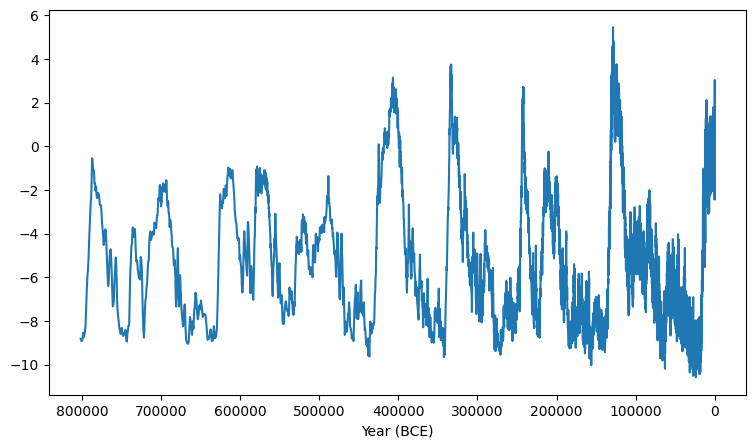
\includegraphics[width=.8\textwidth]{img_input/sample_graph}
\end{center}
\noindent


\textbf{Due to the large magnitude of the years, we will work in terms
  of thousands of years BCE in these problems.} This is taken care of
for you in the provided notebook.






\subsection*{Resources and Submission Instructions}
If you find that you are having trouble with the first couple
problems, we recommend going over the fundamentals of linear algebra
and matrix calculus (see links on website).  The relevant parts of the
\href{https://github.com/harvard-ml-courses/cs181-textbook/blob/master/Textbook.pdf}{cs181-textbook
  notes are Sections 2.1 - 2.7}.  We strongly recommend reading the
textbook before beginning the homework.

We also encourage you to first read the
\href{http://users.isr.ist.utl.pt/~wurmd/Livros/school/Bishop\%20-\%20Pattern\%20Recognition\%20And\%20Machine\%20Learning\%20-\%20Springer\%20\%202006.pdf}{Bishop
  textbook}, particularly: Section 2.3 (Properties of Gaussian
Distributions), Section 3.1 (Linear Basis Regression), and Section 3.3
(Bayesian Linear Regression). (Note that our notation is slightly
different but the underlying mathematics remains the same!).

\textbf{Please type your solutions after the corresponding problems
  using this \LaTeX\ template, and start each problem on a new page.}
You may find the following introductory resources on \LaTeX\ useful:
\href{http://www.mjdenny.com/workshops/LaTeX_Intro.pdf}{\LaTeX\ Basics}
and
\href{https://www.overleaf.com/learn/latex/Free_online_introduction_to_LaTeX_(part_1)}{\LaTeX\ tutorial
  with exercises in Overleaf}

Homeworks will be submitted through Gradescope. You will be added to
the course Gradescope once you join the course Canvas page. If you
haven't received an invitation, contact the course staff through Ed.

\textbf{Please submit the writeup PDF to the Gradescope assignment
  `HW1'.} Remember to assign pages for each question.

\textbf{Please submit your \LaTeX file and code files to the
  Gradescope assignment `HW1 - Supplemental'.} Your files should be
named in the same way as we provide them in the repository,
e.g. \texttt{hw1.pdf}, etc.

%%%%%%%%%%%%%%%%%%%%%%%%%%%%%%%%%%%%%%%%%%%%%
% Problem 1
%%%%%%%%%%%%%%%%%%%%%%%%%%%%%%%%%%%%%%%%%%%%%
\begin{problem}[kNN and Kernels, 35pts]

You will now implement two non-parametric regressions to model temperatures over time.  
% For this problem, you will use the \textbf{same dataset as in Problem 1}.

\vspace{0.5cm}
\noindent\emph{Make sure to include all required plots in your PDF. Passing all test cases does not guarantee that your solution is correct, and we encourage you to write your own. }

\begin{enumerate}
\item 
 Recall that kNN uses a predictor of the form
\[
  f(x^*) = \frac{1}{k} \sum_n y_n \mathbb{I}(x_n \texttt{ is one of k-closest to } x^*),
\]
where $\mathbb{I}$ is an indicator variable. 
\begin{enumerate}

  \item The kNN implementation \textbf{has been provided for you} in the notebook. Run the cells to plot the results for $k=\{1, 3, N-1\}$, where $N$ is the size of the dataset. Describe how the fits change with $k$. Please include your plot in your solution PDF.

  \item Now, we will evaluate the quality of each model \emph{quantitatively} by computing the error on the provided test set. Write Python code to compute test MSE for each value of $k$.  Which solution has the lowest MSE? 
  
\end{enumerate}

\item \textit{Kernel-based regression} techniques are another form of non-parametric regression. Consider a kernel-based
regressor of the form 
\begin{equation*}
  f_\tau(x^*) = \cfrac{\sum_{n} K_\tau(x_n,x^*) y_n}{\sum_n K_\tau(x_n, x^*)}
\end{equation*}
where $\mathcal{D}_\texttt{train} = \{(x_n,y_n)\}_{n = 1} ^N$ are the
training data points, and $x^*$ is the point for which you want to
make the prediction.  The kernel $K_\tau(x,x')$ is a function that
defines the similarity between two inputs $x$ and $x'$. A popular
choice of kernel is a function that decays as the distance between the
two points increases, such as
\begin{equation*}
  K_\tau(x,x') = \exp\left(-\frac{(x-x')^2}{\tau}\right)
\end{equation*}

where $\tau$ represents the square of the lengthscale (a scalar value that
dictates how quickly the kernel decays).  


\begin{enumerate}
    
  \item First, implement the \texttt{kernel\_regressor} function in the notebook, and plot your model for years in the range $800,000$ BC to $400,000$ BC at $1000$ year intervals for the following three values of $\tau$: $1, 50, 2500$. Since we're working in terms of thousands of years, this means you should plot $(x, f_\tau(x))$ for $x = 400, 401, \dots, 800$. \textbf{In no more than 10 lines}, describe how the fits change with $\tau$. Please include your plot in your solution PDF.

  \item Denote the test set as $\mathcal{D}_\texttt{test} = \{(x'_m, y'_m)\}_{m = 1} ^M$.  Write down the expression for MSE of $f_\tau$ over the test set as a function of the training set and test set. Your answer may include $\{(x'_m, y'_m)\}_{m = 1} ^M$, $\{(x_n, y_n)\}_{n = 1} ^N$, and $K_\tau$, but not $f_\tau$.

    \item Compute the MSE on the provided test set for the three values of $\tau$.  Which model yields the lowest MSE? Conceptually, why is this the case? Why would choosing $\tau$ based on $\mathcal{D}_\texttt{train}$ rather than $\mathcal{D}_\texttt{test}$ be a bad idea? 

  \item Describe the time and space complexity of both kernelized regression and kNN with respect to the size of the training set $N$.  How, if at all, does the size of the model---everything that needs to be stored to make predictions---change with the size of the training set $N$?  How, if at all, do the number of computations required to make a prediction for some input $x^*$ change with the size of the training set $N$?.
  

  \item  What is the exact form of $\lim_{\tau \to 0 }f_\tau(x^*)$?
  \end{enumerate}
\end{enumerate}
\end{problem}

\newpage
\begin{solution}
    \begin{figure}
        \centering
        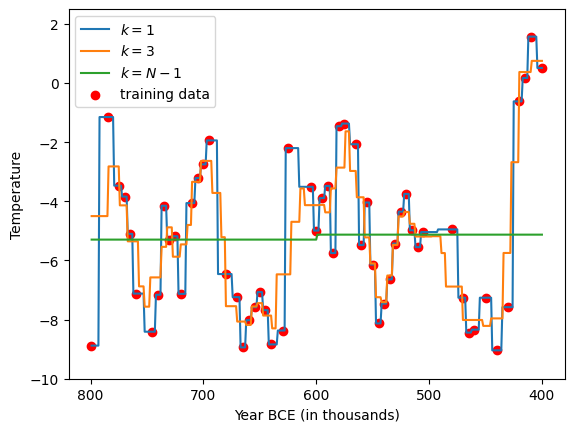
\includegraphics[width=0.7\linewidth]{hw1/images/p1.1a.png}
        \caption{K-Nearest Neighbors Plot}
    \end{figure}
    \begin{tcolorbox}
        \textbf{1. (a)} We can see that at k = 1, the kNN regressor has extremely high variance and low bias. That is, the regression overfits to the training data, with the plotted line snaking through every data point. Thus, at k = 1, we know that the kNN will probably not generalize well since it seems to respond heavily in response to the input data. This makes sense intuitively, since when k = 1, the kNN regressor takes a new input $x$ and simply assigns $\hat{y}$ to the nearest training data point. There is no averaging since there is only 1 neighbor being compared, thus causing the model to overfit to the training data.
        \\
        \\
        At k = N - 1, the kNN regressor outputs an almost flat line that barely changes in response to the training data. Even though the training data follow a roughly sinusoidal shape, the green predicted line doesn't capture this trend at all, instead shooting straight through the middle of all the points. Thus, the model underfits to the training data and has high bias with low variance. This is because at k = N - 1, the model essentially averages all the training data except the farthest point, resulting in the same predicted value for many inputs.
        \\
        \\
        At k = 3, the kNN regressor still captures the general shape of the data, but doesn't perfectly predict every training point. Thus, the model has found a better balance of variance and bias than the previous two $k$ value models and does not overfit or underfit to the data. This makes sense as at k = 3, the model averages the nearest 3 neighbors and uses this as a prediction, which helps capture the local trend of the data but doesn't result in large variation in response to input data due to the averaging.
        \\
        \\
        \textbf{(b)} After computing MSE for all $k$ values from $1$ to $N$, the optimal $k$ value was $k = 1$ with a MSE of 1.741.
    \end{tcolorbox}
    \begin{figure}
        \centering
        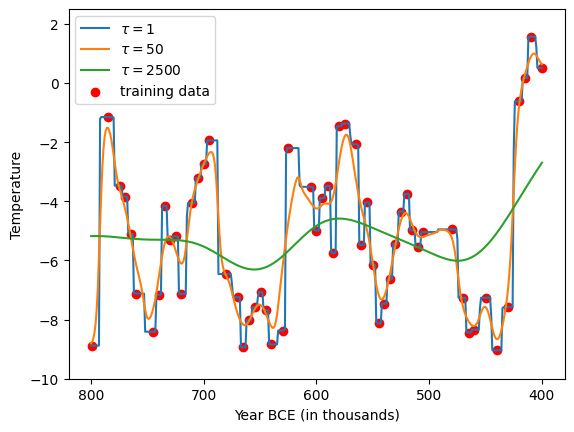
\includegraphics[width=0.7\linewidth]{hw1/images/p1.2a.png}
        \caption{Kernel regression Tau Plot}
    \end{figure}
    \begin{tcolorbox}
        \textbf{2. (a)} When $\tau = 1$, we see the model has high variance and low bias. The model perfectly predicts every training point, but will probably overfit to the training data and not generalize well. When $\tau = 50$, the model has less variance than when $\tau = 1$, but still captures the shape of the data well. When $\tau = 2500$, the model has much higher bias and less variance. Thus, while the shape vaguely resembles the data, the model does not capture the magnitude of fluctuations in data.
        \\
        \\
        \textbf{(b)} Substituting in the formula for $f_{\tau}(x*)$, we can express the MSE as
        $$\text{MSE}(f_\tau) = \frac{1}{M} \sum_{m=1}^M (\cfrac{\sum_{n} K_\tau(x_n,x^*) y_n}{\sum_n K_\tau(x_n, x^*)} - y_m)^2$$
        \\
        \\
        \textbf{(c)} After computing the above MSE formula on the test data, I got an MSE of 1.947 for $\tau = 1$, 1.858 for $\tau = 50$, and 8.333 for $\tau = 2500$. The model that yields the lowest MSE is $\tau = 50$. Conceptually, this is the case since at $\tau = 50$, we find a better balance between the bias and variance of the model. At $\tau = 1$, the model overfits to the training data so it can't generalize as well to the test data. At $\tau = 2500$, the model has too high bias and cannot vary in response to the training data. Thus, the balance of bias and variance at $\tau = 50$ result in a model that captures the fluctuations and shape of the training set without overfitting. Intuitively, the model is good at predicting the distribution of the actual data, rather than predicting just the training values.
        \\
        \\
        If we chose $\tau$ solely on the training data performance, then the mdoel we pick would perfectly predict the training data, but wouldn't necessarily mean accurate predictions on new inputs. Thus, we need to evaluate on the testing set to see how the model generalizes to new data. 
        \\
        \\
        \textbf{(d)} Per Ed \#47, the following analysis is for the space and time complexity it takes to predict one new data point. 
        \\
        \\
        In the kNN algorithm, since we must compare each new input $x*$ to the $k$ nearest neighbors in the training dataset, it follows we must store the entirety of $\mathcal{D}_\texttt{train}$ during inference. Thus, the kNN algorithm has $O(N)$ space complexity. Similarly, to make a new prediction for $x*$, the algorithm calculates the mean of the $k$ nearest points to $x*$. Obtaining the $k$ nearest points can be done in $O(N)$ time and computing the mean takes additional $O(k)$ time. Therefore, the runtime is $O(N + k) = O(N)$ assuming $N >> k$ and O(1) arithmetic.
        \\
        \\
        In kernelized regression, every training point $x_n$ is weighted in the kernel regressor to make a prediction for $x*$. Therefore, we must store all training data $\mathcal{D}_\texttt{train}$ which is $O(N)$ space complexity. Since we perform the kernel function (which is just an O(1) exponentiation) for each training point to compute $f_\tau$, the runtime is O(N) assuming O(1) arithmetic. 
        \\
        \\
        In general, for non-parametric methods like kNN and Kernel regression, we must keep the entirety of the training set when making predictions, since we are not assuming anything about the data. Therefore, the computational complexity and space complexity required to make a prediction for $x*$ increases with the size of $N$.
        \\
        \\
        \textbf{(e)} Recall that the kernel function is
        $$K_\tau(x,x') = \frac{1}{e^{\frac{(x-x')^2}{\tau}}}$$
        Thus,
        $$\lim_{\tau \rightarrow 0} \frac{(x-x')^2}{\tau} = \infty \quad \text{if $x \neq x'$}$$
        $$\lim_{\tau \rightarrow 0}K_\tau(x,x') = 0 \quad \text{if $x \neq x'$}$$
        Therefore, when $\tau \rightarrow 0$, the kernel function approaches 0 for all $x_n$. Any smaller value of the distance $(x-x')^2$ will be infinitely amplified by the $\tau \rightarrow 0$ in the denominator. Therefore, the closest point $x_i$ will have an infinitely larger kernel value compared to the other points and dominate the calculation for $f\tau$. Therefore, when $\tau \rightarrow 0$, $f_\tau$ resembles a 1-NN neighbors regression so
        $$\lim_{\tau \rightarrow 0} f_\tau(x*) = y_i \quad \text{where $i$ is the index of the closest point to $x*$}$$
        
    \end{tcolorbox}
\end{solution}


%%%%%%%%%%%%%%%%%%%%%%%%%%%%%%%%%%%%%%%%%%%%%
% Problem 2
%%%%%%%%%%%%%%%%%%%%%%%%%%%%%%%%%%%%%%%%%%%%%
\newpage
\begin{problem}[Deriving Linear Regression, 20pts]

We now seek to model the temperatures with a parametric method: linear regression. Before we implement anything, let's revisit the mathematical formulation of linear regression.  Specifically, the solution for the least squares linear regression  ``looks'' kind of like a ratio of covariance and
variance terms.  In this problem, we will make that connection more
explicit. \\

\noindent Suppose we have some 2-D data where each observation has the form $(x, y)$ and is independent and identically distributed according  $x \sim p(x)$, $y \sim p(y|x)$. We will consider the process of fitting these data from this distribution with the best linear model
possible, that is a linear model of the form $\hat{y} = wx$ that
minimizes the expected squared loss $E_{x,y}[ ( y - \hat{y} )^2
    ]$.\\

\noindent Note: The notation $E_{x, y}$ indicates an
expectation taken over the joint distribution $p(x,y)$. This essentially just means to treat $x$ and $y$ as random.  

\begin{enumerate}

  \item Derive an expression for the optimal $w$, that is, the $w$
        that minimizes the expected squared loss above.  You should leave
        your answer in terms of moments of the distribution, e.g. terms
        like $E_x[x]$, $E_x[x^2]$, $E_y[y]$, $E_y[y^2]$, $E_{x,y}[xy]$
        etc.

  \item Note that while $x, y$ are data that we have access to, $E_{x, y}[yx]$ is a theoretical constant. Keeping in mind the interpretation of expectations as average values, how could you use observed data $\{(x_n,y_n)\}_{n=1}^N$ to estimate $E_{x, y}[yx]$ and $E_x[x^2]$?

  \item In general, moment terms like $E_{x, y}[yx]$, $E_{x, y}[x^2]$,
        $E_{x, y}[yx^3]$, $E_{x, y}[\frac{x}{y}]$, etc. can easily be
        estimated from the data (like you did above).  If you substitute in
        these empirical moments, how does your expression for the optimal
        $w^*$ in this problem compare with the optimal $\bm{\hat w}$ from Problem 4.3 of HW0?

  \item Many common probabilistic linear regression models assume that
        variables $x$ and $y$ are jointly Gaussian.  Did any of your above
        derivations rely on the assumption that $x$ and $y$ are jointly
        Gaussian?  Why or why not?
\end{enumerate}
\end{problem}

\newpage
\begin{solution}
    \begin{tcolorbox}
        \textbf{1.} Substitution in $\hat{y} = wx$, we can write the expectation as a function of $w$ to minimize:
        $$f(w) = E_{x,y}[ ( y - wx )^2] = E_{x,y}[y^2 - 2ywx + w^2x^2]$$
        By linearity, 
        $$f(w) = E_{x,y}[y^2 - 2ywx + w^2x^2] = E_{x,y}(y^2)- E_{x,y}(2ywx) + E_x(w^2x^2)$$
        $$f(w) = E_{x,y}(y^2)- 2wE_{x,y}(yx) + w^2 E_x(x^2)$$
        Finally, we note that this is a quadratic function in terms of $w$ which points upwards. Thus, we can differentiate with respect to $w$ and set $f'(w) = 0$ to solve for the $w$ that minimizes $f(w)$:
        $$0 = -2E_{x,y}(yx) + 2w E_x(x^2)$$
        $$w = \frac{E_{x,y}(yx)}{E_x(x^2)}$$
        Thus, the optimal $w*$ that minimizes the expected squared loss is
        $$w* = \frac{E_{x,y}(yx)}{E_x(x^2)}$$
    \end{tcolorbox}
    \begin{tcolorbox}
        \textbf{2.} Since expectation is just the theoretical mean value of a random variable, we can take the sample mean of the observed data $\{(x_n,y_n)\}_{n=1}^N$ to approximate the theoretical values:
        $$E_{x, y}[yx] \approx \frac{1}{N} \sum_{n = 1}^N x_ny_n$$
        $$E_x[x^2] \approx \frac{1}{N} \sum_{n=1}^N x_n^2$$
    \end{tcolorbox}
    \begin{tcolorbox}
        \textbf{3.} Substituting in the values derived in part (2) into the expression for part (1), we get:
        $$w* \approx \frac{\frac{1}{N} \sum_{n = 1}^N x_ny_n}{\frac{1}{N} \sum_{n=1}^N x_n^2} = \frac{\sum_{n = 1}^N x_ny_n}{\sum_{n=1}^N x_n^2}$$
    \end{tcolorbox}
    \begin{tcolorbox}
        \textbf{4.} None of my derivations above relied on any assumption of the joint distribution of $x$ and $y$. In part (1), I simply expanded the expression using basic algebra and applied Linearity of Expectation. Note that linearity does not rely on any jointly Gaussian assumption. In part (2), I used the definition of expected value to arrive at the approximations. Therefore, there was no step in any part that assumed a jointly Gaussian distribution of $x$ and $y$. Since we are deriving linear regression purely from the expected squared loss, our derivations should only rely on the existence of the moments of $x$ and $y$, not their distribution.
    \end{tcolorbox}
\end{solution}

%%%%%%%%%%%%%%%%%%%%%%%%%%%%%%%%%%%%%%%%%%%%%
% Problem 3
%%%%%%%%%%%%%%%%%%%%%%%%%%%%%%%%%%%%%%%%%%%%%
\newpage
\begin{problem}[Basis Regression, 30pts]

 Having reviewed the theory, we now implement some linear regression models for the temperature. If we just directly use the data as given to us, we would only have
    a one dimensional input to our model, the year.  To create a more expressive linear
    model, we will introduce basis functions.

\vspace{1em}

\noindent\emph{Make sure to include all required plots in your PDF.}

\begin{enumerate}
  \item
        We will first implement the four basis regressions below. (The first basis has been implemented for you in the notebook as an example.) Note that we introduce an addition transform $f$ (already into the provided notebook) to address concerns about numerical instabilities.
        \begin{enumerate}
          \item $\phi_j(x)= f(x)^j$ for $j=1,\ldots, 9$. $f(x) = \frac{x}{1.81 \cdot 10^{2}}.$
          \item $\phi_j(x) = \exp\left\{-\cfrac{(f(x)-\mu_j)^2}{5}\right\}$ for $\mu_j=\frac{j + 7}{8}$ with $j=1,\ldots, 9$. $f(x) = \frac{x}{4.00 \cdot 10^{2}}.$
          \item $\phi_j(x) =  \cos(f(x) / j)$ for $j=1, \ldots, 9$. $f(x) = \frac{x}{1.81}$.
          \item $\phi_j(x) = \cos(f(x) / j)$ for $j=1, \ldots, 49$. $f(x) = \frac{x}{1.81 \cdot 10^{-1}}$. \footnote{For the trigonometric bases (c) and (d), the periodic nature of
                  cosine requires us to transform the data such that the
                  lengthscale is within the periods of each element of our basis.}
        \end{enumerate}

        {\footnotesize * Note: Please make sure to add a bias term for
        all your basis functions above in your implementation of the
        \verb|make_basis|.}

        Let
        $$ \mathbf{\phi}(\mathbf{X}) =
          \begin{bmatrix}
            \mathbf{\phi}(x_1) \\
            \mathbf{\phi}(x_2) \\
            \vdots             \\
            \mathbf{\phi}(x_N) \\
          \end{bmatrix} \in \mathbb{R}^{N\times D}.$$
        You will complete the \verb|make_basis| function which must return
        $\phi(\mathbf{X})$ for each part
        (a) - (d). You do NOT need to submit this
        code in your \LaTeX writeup.

        Then, create a plot of the fitted
        regression line for each basis against a scatter plot
        of the training data. Boilerplate plotting code is provided in the
        notebook---you will only need to finish up a part of it.
        \textbf{All you need to include
          in your writeup for this part are these four plots.}

        \item
          Now we have trained each of our basis regressions. For each basis
          regression, compute the MSE on the test set.  Discuss: do any of the
          bases seem to overfit?  Underfit?  Why?


    \item Briefly describe what purpose the transforms $f$ serve: why are they helpful?

    \item As in Problem 1, describe the space and time complexity of linear regression.  How does what is stored to compute predictions change with the size of the training set $N$ and the number of features $D$?  How does the computation needed to compute the prediction for a new input depend on the size of the training set $N$?  How do these complexities compare to those of the kNN and kernelized regressor?

    \item Briefly compare and constrast the different regressors: kNN,
          kernelized regression, and linear regression (with bases).  Are some
          regressions clearly worse than others?  Is there one best
          regression?  How would you use the fact that you have these multiple
          regression functions?

  \end{enumerate}
  Note:
  Recall that we are using a
  different set of inputs $\mathbf{X}$ for each basis (a)-(d).
  Although it may seem as though this prevents us from being able
  to directly compare the MSE since we are using different data,
  each transformation can be considered as being a part of our model.
  Contrast this with transformations (such as standardization) that cause the variance of the target $\mathbf{y}$ to be different; in these cases the
  MSE can no longer be directly compared.
\end{problem}

\newpage 
\begin{solution}
    \textbf{1.} \begin{figure}[H]
        \centering
        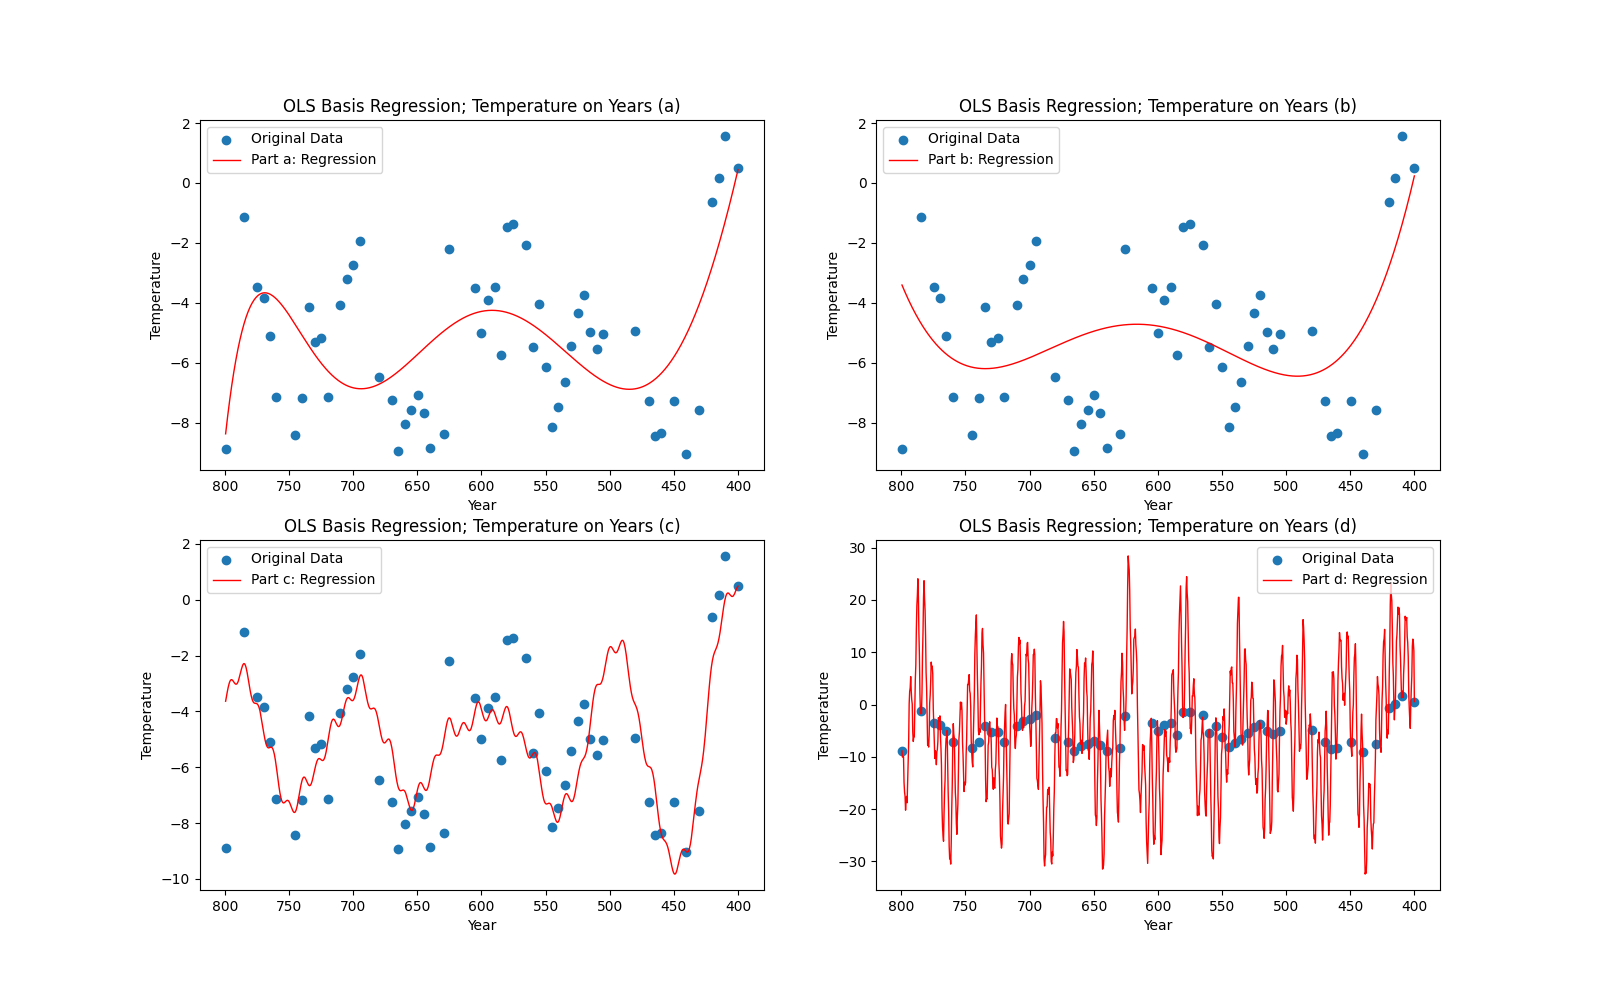
\includegraphics[width=0.9\linewidth]{hw1/images/p3.1.png}
        \caption{Basis regression lines}
        \label{fig:enter-label}
    \end{figure}
    \begin{tcolorbox}
        \textbf{2.} The MSEs are 7.956 for part a, 8.708 for part b, 5.976 for part c, and 58.906 for part d. The base in part (d) seems to overfit. This is evident due to the extremely high variance which causes the erratic peaks and valleys in the regression line. The reason for this could be because the basis expands the dimension of inputs too much (by 50 instead of 10 like the other bases). This level of granularity in the inputs results in the model overreacting to variation and noise in individual training data points. As such, the variance is far too high and the model does not generalize well on new data, as evidenced by its much higher MSE, and could benefit from a regularization scheme. On the other hand, the basis in (b) seems to underfit. While the shape of the line still vaguely matches the trends of the data, the line does not react enough to the variation of the data. I would hypothesize that this is due to the 9 Gaussian features not being enough to capture the relatively complex trends in the training data. Thus, the model is too simple and the bias is too high, causing it to underfit. Finally, the basis in part (c) seems to fit the best, with the lowest MSE. I would hypothesize that the periodicity of the 9 cosine functions naturally makes this basis a great fit for the periodic trends in the training data. 
    \end{tcolorbox}
    \begin{tcolorbox}
        \textbf{3.} In a simple linear regression model with no basis transformations, there is little to no flexibility-- if the data simply follows a trend which is nonlinear, then regression model will struggle with high bias due to its simplicity. Thus, basis functions allow us to transform the feature space into one that is better suited for the trends we observe, such as polynomial curves, periodic data, or other nonlinear relationships.
    \end{tcolorbox}
    \begin{tcolorbox}
        \textbf{4.} Again, the following analysis is for the space and time complexity required to predict one new input. That is, I assume that the optimal weights $w$ are already found and all that remains is the matrix multiplication of $x*$ and $w$. That is, we must perform
        $$y = wx*$$
        Let us denote the dimension of input after applying the basis as $d$. We know that the weights $w$ are a 1 dimensional vector $d$ and notably, we don't need the actual training data during inference since we have already used it to calibrate the parameters $w$. Thus, all we need is $w$ so the space complexity of this is $O(d)$. The runtime of this regression is split into two parts: applying the basis, and the dot product $wx*$. Applying a $d$ dimensional expansion to the input takes $O(d)$ time assuming $O(1)$ arithmetic. Then, the dot product of $wx*$ takes $O(d)$ time as well since the two vectors are $d$ length. Therefore, the total runtime is $O(d)$. 
        \\
        \\
        Compared to the nonparametric counterparts such as the kNN and kernelized regressor, the parametric basis regression has much less space overhead and runtime requirements at $O(d)$ compared to $O(N)$ (assuming $N >> d$ which is common). 
    \end{tcolorbox}
    \begin{tcolorbox}
        For the linear basis regression, we don't need to store the entire training dataset during inference to compare our new input with-- we only need to use the training dataset to find optimal $w$ before prediction. As such, the runtime and space requirements of the basis regression method is much less (at $N >> d$) since we only need to apply the basis and perform a dot product of two vectors, which can be optimized. In contrast, the non parametric methods need to use all $N$ training samples to output a new prediction, which is both slow and costly when the training dataset is large. However, it is worth noting that basis regression has an overhead cost of computing optimal $w = (X^TX)^{-1}X^Ty$ while the kNN and kernelized methods don't require such an overhead. However, since this is computed before any prediction, the linear basis regression likely still has better runtime. 
        \\
        \\
        While it is clear that the linear basis regression is better in terms of space overhead and runtime, the nonparametric kNN and kernelized regressor had much better accuracy. Importantly, I note that the methods are comparable since they were evaluated using the same metric on the same training and validation sets, with no additional transformations other than the applied basis in the linear regression. The MSE of the kNN and kernelized regression was around 1.7-1.8 whereas the best MSE of the bases was around 6.
        \\
        \\
        Thus, there seems to be a tradeoff here in terms of resources and accuracy. The nonparametric basis regression has lower space and runtime complexity due to not needing to keep all training data on hand when making a new prediction, but thus is less accurate. In general, there is no one best model of regression. The advantage of multiple models is that we can use techniques like cross validation to find the optimal model for our needs.
    \end{tcolorbox}
\end{solution}

%%%%%%%%%%%%%%%%%%%%%%%%%%%%%%%%%%%%%%%%%%%%%
% Problem 4
%%%%%%%%%%%%%%%%%%%%%%%%%%%%%%%%%%%%%%%%%%%%%
\begin{problem}[Probablistic Regression and Regularization, 30pts]

Finally, we will preview Bayesian regression and explore its connection to regularization for linear models. Then, we will fit a regularized model to the temperature data. Although the content is related, you do not need to know the material from the lectures on frequentist model selection and Bayesian model selection to solve this problem.  \\

\noindent Recall that the probabilistic version of linear regression states that 
\[y_n = \boldw^\top\boldx_n + \epsilon_n, \quad \epsilon_n \sim \mathcal{N}(0, \sigma^2)\]
In Bayesian regression, we impose a prior $p(\boldw)$ on the weights and  fit the weights $\boldw$ through maximizing the posterior likelihood
\[p(\boldw | \boldX, \boldy) = \frac{p(\bold y | \boldw, \boldX)p(\boldw)}{p(\boldy | \boldX)}\]
Note: since we maximize with respect to $\boldw$, it suffices to just maximize the numerator.

\begin{enumerate}
    \item Suppose $\boldw \sim \mathcal{N}(\mathbf{0},\frac{\sigma^2}{\lambda}\boldI)$. Show that maximizing the posterior likelihood is equivalent to minimizing 
    \[\mathcal{L}_{ridge}(\boldw) = \frac{1}{2}||\boldy -\bold X\boldw||_2^2 + \frac{\lambda}{2}||\boldw||_2^2.\] 
    Note that minimizing $\mathcal{L}_{ridge}(\boldw)$ is exactly what ridge regression does.
    
    Hint: You don't need to solve for the maximizer/minimizer to show that the optimization problems are equivalent.
    
    \item Solve for the value of $\boldw$ that minimizes $\mathcal L_{ridge}(\boldw)$.

    \item The Laplace distribution has the PDF
   \[L(a,b) =\frac{1}{2b} \exp\left(-\frac{|x - a|}{b}\right)\]
Show that if all $w_d \sim L\left(0,\frac{2\sigma^2}{\lambda}\right)$, maximizing the posterior likelihood is equivalent to minimizing 
\[\mathcal{L}_{lasso}(\boldw) = \frac{1}{2}||\boldy -\bold X\boldw||_2^2  + \frac{\lambda}{2}||\boldw||_1.\] 
Note that minimizing $\mathcal{L}_{lasso}(\boldw)$ is exactly what LASSO regression does.

    \item Why is there no general closed form for the LASSO estimator, i.e. the value of $\boldw$ that minimizes $\mathcal{L}_{ridge}(\boldw)$?

    \item Since there is no general closed form for LASSO, we use numerical methods for estimating $\boldw$. One approach is to use \textit{coordinate descent}, which works as follows: 
    \begin{enumerate}
        \item Initialize $\boldw=\boldw_0$.
        \item For each $d=1, \ldots, D$ do the following 2 steps consecutively:
        \begin{enumerate}
            \item Compute $\rho_d = \tilde{\boldx}_d^\top(\boldy - (\boldX \boldw - w_d \tilde{\boldx}_d))$. We define $\tilde{\boldx}_d$ as the $d$-th column of $\boldX$.

            \item If $d=1$, set $w_1 = \frac{\rho_1}{||\tilde{\boldx}_1||^2_2}$. Otherwise if $d\ne 1$, compute $w_d = \frac{\text{sign}(\rho_d)\max\left\{|\rho_d|-\frac{\lambda}{2}, 0\right\}}{||\tilde{\boldx}_d||^2_2}$.
        \end{enumerate}
        \item Repeat step (b) until convergence or the maximum number of iterations is reached.
    \end{enumerate} 

    Implement the \texttt{find\_lasso\_weights} function according to the above algorithm, letting $\boldw_0$ be a vector of ones and the max number of iterations be 5000. Then, fit models with $\lambda=1, 10$ to basis (d) from Problem 3, plot the predictions, and compute the MSE's. You will need to do some preprocessing, but a completed helper function for this is already provided. How do the graphs and errors compare to those for the unregularized basis (d) model? 


\end{enumerate}

\end{problem}

\newpage
\begin{solution}
    \begin{tcolorbox}
        \textbf{1.} Per the hint, we will choose to maximize across the numerator since the denominator is constant with respect to $w$. This leads us to
        $$p(\boldw | \boldX, \boldy) \propto p(\bold y | \boldw, \boldX)p(\boldw)$$
        Therefore, if we have Gaussian prior $\boldw \sim \mathcal{N}(\mathbf{0},\frac{\sigma^2}{\lambda}\boldI)$, then
        $$p(\boldw) = (\frac{\lambda}{2\pi\sigma^2})^{\frac{D}{2}} \exp(- \frac{\lambda}{2\sigma^2} \boldw^\top\boldw) \propto \exp(-\frac{\lambda}{2\sigma^2} ||\boldw||^2_2)$$
        Then, from $y_n = \boldw^\top\boldx_n + \epsilon_n$ and  $\epsilon_n \sim \mathcal{N}(0, \sigma^2)$, we have 
        $$y_n | \boldw^\top\boldx_n, \sigma^2  \sim \mathcal{N}(\boldw^\top\boldx_n, \sigma^2)$$
        Thus, using the normal PDF but dropping the constants, we get the likelihood
        $$p(\bold y | \boldw, \boldX) \propto \prod_{n=1}^N \exp(- \frac{(y_n - \boldw^\top\boldx_n)^2}{2\sigma^2}) = \exp(- \frac{1}{2\sigma^2}\sum_{n=1}^N (y_n - \boldw^\top\boldx_n)^2)$$
        $$\propto  \exp(- \frac{1}{2\sigma^2} ||\boldy - \boldX\boldw||^2_2)$$
        Therefore,
        $$p(\boldw | \boldX, \boldy) \propto \exp(- \frac{1}{2\sigma^2} ||\boldy - \boldX\boldw||^2_2) \cdot \exp(-\frac{\lambda}{2\sigma^2} ||\boldw||^2_2)$$ 
        $$\propto \exp(-\frac{1}{2\sigma^2} ||\boldy - \boldX\boldw||^2_2 -\frac{\lambda}{2\sigma^2} ||\boldw||^2_2)$$
        We can then take the log likelihood to get:
        $$\log p(\boldw | \boldX, \boldy) \propto -\frac{1}{\sigma^2} (\frac{1}{2}||\boldy - \boldX\boldw||^2_2 +\frac{\lambda}{2} ||\boldw||^2_2)$$
        Notice that the parentheses inner expression matches the expression for $\mathcal{L}_{ridge}(\boldw)$. Moreover, we know that $-\frac{1}{\sigma^2}$ is a negative constant. Therefore, to maximize $p(\boldw | \boldX, \boldy)$, we must minimize the expression
        $$\frac{1}{2}||\boldy - \boldX\boldw||^2_2 +\frac{\lambda}{2} ||\boldw||^2_2$$
        Which is the exact same goal as minimizing
        $$\mathcal{L}_{ridge}(\boldw) = \frac{1}{2}||\boldy -\bold X\boldw||_2^2 + \frac{\lambda}{2}||\boldw||_2^2$$
    \end{tcolorbox}
    \begin{tcolorbox}
        \textbf{2.} To find the value of $\boldw$ that minimizes $\mathcal{L}_{ridge}(\boldw)$, we simply take the derivative with respect to $\boldw$ and set the expression equal to 0.
        $$\frac{d\mathcal{L}_{ridge}(\boldw)}{d\boldw} = -\boldX^\top\boldy + \boldX^\top\boldX\boldw + \lambda\boldy$$
        $$-\boldX^\top\boldy + \boldX^\top\boldX\boldw + \lambda\boldy = 0$$
        We then solve for the optimal $\boldw$, which is
        $$\boldw = (\boldX^\top\boldX + \lambda\boldI)^{-1}\boldX^\top\boldy$$
    \end{tcolorbox}
    \begin{tcolorbox}
        \textbf{3.} If we know that all
        $$w_d \sim L\left(0,\frac{2\sigma^2}{\lambda}\right)$$
        Then we can express the likelihood $p(\boldw)$ using the Laplace PDF as
        $$p(\boldw) = \prod_{d = 1}^D \frac{\lambda}{4\sigma^2}\exp(-\frac{\lambda|w_d|}{2\sigma^2})$$
        $$ = \left(\frac{\lambda}{4\sigma^2}\right)^{D} \exp(-\frac{\lambda}{2\sigma^2} \sum_{d = 1}^D |w_d|)$$
        $$ = \left(\frac{\lambda}{4\sigma^2}\right)^{D} \exp(-\frac{\lambda}{2\sigma^2} ||\boldw||_1)$$
        We also know form part (1) that
        $$p(\bold y | \boldw, \boldX) \propto  \exp(- \frac{1}{2\sigma^2} ||\boldy - \boldX\boldw||^2_2)$$
        Therefore, as before, we have:
        $$p(\boldw | \boldX, \boldy) \propto p(\bold y | \boldw, \boldX)p(\boldw)$$
        Dropping constants, we have
        $$p(\boldw | \boldX, \boldy) \propto \exp(- \frac{1}{2\sigma^2} ||\boldy - \boldX\boldw||^2_2 \cdot \exp(-\frac{\lambda}{2\sigma^2} ||\boldw||_1)$$
        $$p(\boldw | \boldX, \boldy) \propto \exp(- \frac{1}{2\sigma^2} ||\boldy - \boldX\boldw||^2_2-\frac{\lambda}{2\sigma^2} ||\boldw||_1)$$
        $$p(\boldw | \boldX, \boldy) \propto \exp(-\frac{1}{\sigma^2} (\frac{1}{2}||\boldy - \boldX\boldw||^2_2 +\frac{\lambda}{2} ||\boldw||_1))$$
        Taking the log as before,
        $$\log p(\boldw | \boldX, \boldy) \propto-\frac{1}{\sigma^2} (\frac{1}{2}||\boldy - \boldX\boldw||^2_2 +\frac{\lambda}{2} ||\boldw||_1)$$
        By similar logic, maximizing the likelihood $p(\boldw | \boldX, \boldy)$ means minimizing $\frac{1}{2}||\boldy - \boldX\boldw||^2_2 +\frac{\lambda}{2} ||\boldw||_1$ due to the negative constant. Note that this is the exact same action as minimizing
        $$\mathcal{L}_{lasso}(\boldw) = \frac{1}{2}||\boldy -\bold X\boldw||_2^2  + \frac{\lambda}{2}||\boldw||_1$$
    \end{tcolorbox}
    \begin{tcolorbox}
        \textbf{4.} We cannot solve for the value of $\boldw$ that minimizes $\mathcal{L}_{lasso}$ since the L1 Norm regularization penalty is not differentiable when we have any $w_d = 0$ (because of the term $|w_d|$). Thus, there is no general closed form for LASSO.
    \end{tcolorbox}
    \begin{figure}[H]
        \centering
        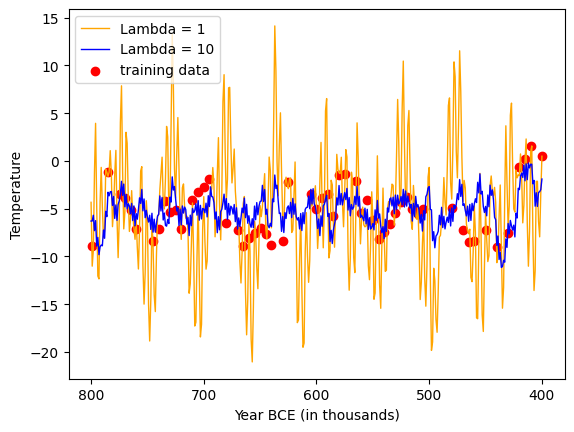
\includegraphics[width=0.9\linewidth]{hw1/images/p4.5.png}
        \caption{LASSO Regression Plot}
    \end{figure}
    \begin{tcolorbox}
       After plotting and computing the MSE for each lambda, I got an MSE of 30.060 for $\lambda = 1$ and an MSE of 15.618 for $\lambda = 10$. Compared the plot of the (d) basis, we see that the $\lambda = 1$ plot is similar in shape due to its high variance, but the magnitude of its fluctuations are smaller. As such, the $\lambda = 1$ model had a lower MSE than the part (d) model. The $\lambda = 10$ regression fits to the data much better than $\lambda = 1$ or part (d) regression. The model does not overfit to the data as much as the part (d) regression (the variance is much lower). Despite this, the $\lambda = 10$ model achieved a much smaller MSE than the part (d) model. This reduction in variance can be attributed to the regularization term introduced which penalizes overly large weights.
    \end{tcolorbox}
\end{solution}


%%%%%%%%%%%%%%%%%%%%%%%%%%%%%%%%%%%%%%%%%%%%%
% Name and Calibration
%%%%%%%%%%%%%%%%%%%%%%%%%%%%%%%%%%%%%%%%%%%%%
\newpage
\subsection*{Name}
Jaray Liu
\subsection*{Collaborators and Resources}
Whom did you work with, and did you use any resources beyond cs181-textbook and your notes?
Zihongbo Wang


\end{document}
